\chapter{Week 2}
\section{Linear Regression}

	\subsection{Introduction to Regression}	
	
	Hello and welcome! In this video we'll be giving a brief introduction to regression. So let's get started. Look at this data set. It's related to co2 emissions from different cars. 
	It includes engine size, number of cylinders, fuel consumption, and co2 emission from various automobile models. 
	
	The question is: given this data set can we predict the co2 emission of a car using other fields such as engine size or cylinders? Let's assume we have some historical data from different cars and assume that a car such as in row 9 has not been manufactured yet, but we're interested in estimating its approximate co2 emission after production. Is it possible? 
	
	We can use regression methods to predict a continuous value such as co2 emission using some other variables. Indeed regression is t\textbf{he process of predicting a continuous value}. 
	In regression there are \textbf{two types of variables}: a \textbf{dependent variable} and \textbf{one or more independent variables}. 
	
	The dependent variable can be seen as the state, target, or final goal we study and try to predict. 
	And the independent variables, also known as explanatory variables, can be seen as the causes of those states. The independent variables are shown conventionally by X and the dependent variable is notated by Y.
	
	A regression model relates Y or the dependent variable to a function of X i.e. the independent variables. 
	
	The key point in the regression is that our dependent value should be continuous and cannot be a discrete value. 
	However, the independent variable, or variables, can be measured on either a categorical or continuous measurement scale. 
	
	So, what we want to do here is to use the historical data of some cars using one or more of their features and from that data make a model. We use regression to build such a regression estimation model; then the model is used to predict the expected co2 emission for a new or unknown car. 
	
	Basically there are two types of regression models \textbf{simple regression} and \textbf{multiple regression}. Simple regression is when \textbf{one independent variable is used} to estimate a dependent variable. It \textbf{can be either linear or non-linear}. 
	For example, predicting co2 emission using the variable of engine size. 
	Linearity of regression is based on the nature of relationship between independent and dependent variables. When \textbf{more than one independent variable is present} the process is called \textbf{multiple linear regression}. For example, predicting co2 emission using engine size and the number of cylinders in any given car. Again, depending on the relation between dependent and independent variables it can be either linear or non-linear regression. 
	
	Let's examine some sample applications of regression. 
	Essentially we use regression when we want to estimate a continuous value. For instance, one of the applications of regression analysis could be in the area of sales forecasting. You can try to predict a sales person's total yearly sales from independent variables such as age, education, and years of experience. 
	It can also be used in the field of psychology, for example, to determine individual satisfaction, based on demographic and psychological factors. We can use regression analysis to predict the price of a house in an area, based on its size number of bedrooms, and so on. We can even use it to predict employment income for independent variables such as hours of work, education, occupation, sex, age, years of experience, and so on. 
	
	Indeed, you can find many examples of the usefulness of regression analysis in these and many other fields or domains, such as finance, healthcare, retail, and more. We have many regression algorithms, each of them has its own importance and a specific condition to which their application is best suited. And while we've covered just a few of them in this course, it gives you enough base knowledge for you to explore different regression techniques. 
	
	\subsection{Simple Linear Regression}
	
	
	In this video, we'll be covering linear regression. You don't need to know any linear algebra to understand topics in linear regression. This high-level introduction will give you enough background information on linear regression to be able to use it effectively on your own problems. So let's get started.
	
	Let's take a look at this data set. It's related to the Co2 emission of different cars. It includes engine size, cylinders, fuel consumption and Co2 emissions for various car models. The question is, given this data set, can we predict the Co2 emission of a car using another field such as engine size? 
	
	Quite simply, yes. We \textbf{can use linear regression to predict a continuous value such as Co2 emission by using other variables}. Linear regression is the approximation of a linear model used to describe the relationship between two or more variables. In simple linear regression, there are two variables, a dependent variable and an independent variable.
	The \textbf{key point} in the linear regression is that our dependent value \textbf{should be continuous and cannot be a discrete value}. However, the independent variables can be measured on either a categorical or continuous measurement scale. 
	
	There are two types of linear regression models. They are simple regression and multiple regression. Simple linear regression is when one independent variable is used to estimate a dependent variable. For example, predicting Co2 emission using the engine size variable. When more than one independent variable is present the process is called multiple linear regression, for example, predicting Co2 emission using engine size and cylinders of cars. Our focus in this video is on simple linear regression. 
	
	Now let's see how linear regression works. Okay, so let's look at our data set again. To understand linear regression, we can plot our variables here. We show engine size as an independent variable and emission as the target value that we would like to predict. A scatter plot clearly shows the relation between variables where changes in one variable explain or possibly cause changes in the other variable. Also, it indicates that these variables are linearly related. With linear regression \textbf{you can fit a line through the data}. For instance, as the engine size increases, so do the emissions. With linear regression you can model the relationship of these variables. A good model can be used to predict what the approximate emission of each car is.
	
	How do we use this line for prediction now?
	
	Let us assume for a moment that the line is a good fit of the data. We can use it to predict the emission of an unknown car. For example, for a sample car with engine size $2.4$, you can find the emission is $214$.
	
	Now, let's talk about what the fitting line actually is.
	
	We're going to predict the target value y. In our case using the independent variable engine size represented by $x_{1}$. The fit line is shown traditionally as a polynomial. In a simple regression problem, a single $x$, the form of the model would be $\theta_{0} + \theta_{1}x_{1}$. In this equation, y hat ($\hat{y}$) is the dependent variable of the predicted value. And $x_{1}$ is the independent variable.
	
	Theta 0 ($\theta_{0}$) and theta 1 ($\theta_{1}$) are the parameters of the line that we must adjust. Theta 1 is known as the slope or gradient of the fitting line and theta 0 is known as the intercept.
	
	Theta 0 ($\theta_{0}$) and theta 1 ($\theta_{1}$)are also called the \textbf{coefficients of the linear equation}.
	
	You can interpret this equation as y hat being a function of x1, or y hat being dependent of x1. How would you draw a line through the points? And how do you determine which line fits best?
	
	Linear regression estimates the coefficients of the line. This means we must calculate theta 0 and theta 1 to find the best line to fit the data. This line would best estimate the emission of the unknown data points. 
	
	Let's see how we can find this line or, to be more precise, how we can adjust the parameters to make the line the best fit for the data. For a moment, let's assume we've already found the best fit line for our data. Now, let's go through all the points and check how well they align with this line. Best fit here means that if we have, for instance, a car with engine size $x1 = 5.4$ and actual $Co2 = 250$, its Co2 should be predicted very close to the actual value, which is $y = 250$ based on historical data. But if we use the fit line, or better to say using our polynomial with known parameters to predict the Co2 emission, it will return $\hat{y}= 340$. Now if you compare the actual value of the emission of the car with what we've predicted using our model, you will find out that we have a $90$ unit error. This means our prediction line is not accurate. This error is also called the \textbf{residual error}. So we can say the \textbf{error is the distance from the data point to the fitted regression line}.
	
	\begin{equation}
		MSE = \frac{1}{n} \sum_{i=1}^{n}(y_i - \hat{y}_i)^{2}
	\end{equation}
	The mean of all residual errors shows how poorly the line fits with the whole data set. Mathematically it can be shown by the equation \textbf{Mean Squared Error}, shown as \textbf{MSE}. Our objective is to \textbf{find a line where the mean of all these errors is minimized}. In other words, the mean error of the prediction using the fit line should be minimized. Let's reword it more technically. The \textbf{objective of linear regression}, is to \textbf{minimize this MSE equation and to minimize it, we should find the best parameters theta 0 and theta 1}. Now the question is \textbf{how to find theta 0 and theta 1 in such a way that it minimizes this error?}
	
	How can we find such a perfect line? Or said another way, how should we find the best parameters for our line? Should we move the line a lot randomly and calculate the MSE value every time and choose the minimum one? Not really. Actually, we have \textbf{two options here}. Option one, we can use a \textbf{mathematic approach}, or option two, we can use an \textbf{optimization approach}. Let's see how we could easily use a mathematic formula to find the theta 0 and
	
	As mentioned before, theta 0 and theta 1 in the simple linear regression are the coefficients of the fit line. We can use a simple equation to estimate these coefficients. That is, given that it's a simple linear regression with only two parameters, and knowing that theta 0 and theta 1 are the intercept and slope of the line, we can estimate them directly from our data. It requires that we calculate the mean of the independent and dependent or target columns from the data set. Notice that all of the data must be available to traverse and calculate the parameters. It can be shown that the intercept and slope can be calculated using these equations.
	
	We can start off by estimating the value for theta 1. This is how you can find the slope of a line based on the data. X bar is the average value for the engine size in our data set. Please consider that we have nine rows here, rows 0 to 8. First we calculate the average of x1 and of y, then we plug it into the slope equation to find theta 1.
	
	The xi and yi in the equation refer to the fact that we need to repeat these calculations across all values in our data set. And i refers to the ith value of x or y. Applying all values, we find theta 1 equals 39. It is our second parameter. It is used to calculate the first parameter which is the intercept of the line.
	
	Now we can plug theta 1 into the line equation to find theta 0. It is easily calculated hat theta 0 equals 125.74. So these are the two parameters for the line, where theta 0 is also called the bias coefficient, and theta 1 is the coefficient for the Co2 emission column.
	
	As a side note, you really don't need to remember the formula for calculating these parameters, as \textbf{most of the libraries used for machine learning in Python}, R and Scala \textbf{can easily find these parameters for you}. But it's always good to understand how it works. Now, we can write down the polynomial of the line.
	
	\begin{equation}
		\hat{y} = \theta_{1}x +\theta_{0}
				= 39x + 125.74
	\end{equation}
	
	So we know how to find the best fit for our data and its equation. Now the question is how can we use it to predict the emission of a new car based on its engine size?
	
	After we found the parameters of the linear equation, making predictions is as simple as solving the equation for a specific set of inputs.
	
	Imagine we are predicting Co2 emission, or y, from engine size, or x for the automobile in record number 9. Our linear regression model representation for this problem would be $\hat{y} = \theta_{1}x +\theta_{0}$. Or if we map it to our data set, it would be $Co2Emission =\theta_{0} + \theta_{1} EngineSize$.
	
	As we saw, we can find theta 0, theta 1 using the equations that we just talked about. Once found, we can plug in the equation of the linear model. For example, let's use $\theta_{0} = 125$ and $\theta_{1} = 39$. So we can rewrite the linear model as $Co2Emission = 125 + 39 EngineSize$. Now let's plug in the 9th row of our data set and calculate the Co2 emission for a car with an engine size of 2.4. So $Co2Emission = 125 + 39 x 2.4$. Therefore, we can predict that the Co2Emission for this specific car would be $218.6$. 
	
	Let's talk a bit about why linear regression is so useful. Quite simply, it is the most basic regression to use and understand. In fact, one reason why linear regression is so useful is that \textbf{it's fast}. It also \textbf{doesn't require tuning of parameters}. So something like tuning the K parameter and K nearest neighbors, or the learning rate in neural networks isn't something to worry about. Linear regression is also \textbf{easy to understand}, and \textbf{highly interpretable}.
	
	\subsection{Model Evaluation in Regression Models}
	
    We'll be covering model evaluation. So let's get started. The goal of regression is to build a model to accurately predict an unknown case. To this end, we have to perform regression evaluation after building the model. 
    
    We'll introduce and discuss two types of evaluation approaches that can be used to achieve this goal. 
    These approaches are:
    
    \begin{itemize}
    	\item Train and test on the same dataset

    	\item Train/test split. 

    \end{itemize}  
     
    We'll talk about what each of these are, as well as the pros and cons of using each of these models. Also, we'll introduce some metrics for accuracy of regression models. 
    
    Let's look at the first approach. When considering evaluation models, we clearly want to choose the one that will give us the most accurate results. So, the question is, how can we calculate the accuracy of our model? In other words, how much can we trust this model for prediction of an unknown sample using a given dataset and having built a model such as linear regression? 
    
    One of the solutions is to select a portion of our dataset for testing. For instance, assume that we have 10 records in our dataset. We use the entire dataset for training, and we build a model using this training set. Now, we select a small portion of the dataset, such as row number six to nine, but without the labels. This set is called a \textbf{test set}, which has the labels, but the labels are not used for prediction and is used only as ground truth. The \textbf{labels are called actual values of the test set}. Now we pass the feature set of the testing portion to our built model and predict the target values. Finally, we compare the predicted values by our model with the actual values in the test set. 
    
    This indicates how accurate our model actually is. There are different metrics to report the accuracy of the model, but most of them work generally based on the similarity of the predicted and actual values. 
    
    Let's look at one of the simplest metrics to calculate the accuracy of our regression model. 
    
    \begin{equation}
    	Error = \frac{1}{n} \sum_{j=1}^{n}|y_{i}-\hat{y}| 
    \end{equation}
    
    As mentioned, we just compare the actual values y with the predicted values, which is noted as $\hat{y}$ for the testing set. The \textbf{error of the model is calculated as the average difference between the predicted and actual values for all the rows}. We can write this error as an equation. 
    
    So, the first evaluation approach we just talked about is \textbf{the simplest one, train and test on the same dataset}. Essentially, the name of this approach says it all. You train the model on the entire dataset, then you test it using a portion of the same dataset. In a general sense, when you test with a dataset in which you know the target value for each data point, you're able to obtain a percentage of accurate predictions for the model. 
    This evaluation approach would most likely \textbf{have a high training accuracy and the low out-of-sample accuracy since the model knows all of the testing data points from the training}. What is \textbf{training accuracy} and \textbf{out-of-sample accuracy}? 
    
    We said that training and testing on the same dataset produces a high training accuracy, but what exactly is training accuracy?
    
    Training accuracy is the \textbf{percentage of correct predictions that the model makes when using the test dataset}. However, a high training accuracy isn't necessarily a good thing. For instance, having a high training accuracy \textbf{may result in an over-fit the data}. 
    This means that the model is overly trained to the dataset, which \textbf{may capture noise and produce a non-generalized model}. 
    
    Out-of-sample accuracy is the \textbf{percentage of correct predictions that the model makes on data that the model has not been trained on}. Doing a train and test on the same dataset will most likely have low out-of-sample accuracy due to the likelihood of being over-fit. \textbf{It's important that our models have high out-of-sample accuracy because the purpose of our model is, of course, to make correct predictions on unknown data}. So, how can we improve out-of-sample accuracy? 
    
    One way is to use another evaluation approach called \textbf{train/test split}. In this approach, we select a portion of our dataset for training, for example, row zero to five, and the rest is used for testing, for example, row six to nine. The model is built on the training set. Then, the test feature set is passed to the model for prediction. Finally, the predicted values for the test set are compared with the actual values of the testing set. 
    The second evaluation approach is called train/test split. Train/test split involves splitting the dataset into training and testing sets respectively, which are mutually exclusive. After which, you train with the training set and test with the testing set. This\textbf{ will provide a more accurate evaluation on out-of-sample accuracy} because the testing dataset is not part of the dataset that has been used to train the data. It is \textbf{more realistic for real-world problems}. This means that we know the outcome of each data point in the dataset, making it great to test with. 
    Since this data has not been used to train the model, the model has no knowledge of the outcome of these data points. So, in essence, \textbf{it's truly out-of-sample testing}. 
    
    However, please ensure that you train your model with the testing set afterwards, as you don't want to lose potentially valuable data. 
    The issue with train/test split is that \textbf{it's highly dependent on the datasets on which the data was trained and tested}.
    The variation of this causes train/test split to have a better out-of-sample prediction than training and testing on the same dataset, but it still has some problems due to this dependency. 
    
    Another evaluation model, called \textbf{K-fold cross-validation}, resolves most of these issues.
    How do you fix a high variation that results from a dependency? Well, you average it. Let me explain the basic concept of K-fold cross-validation to see how we can solve this problem. 
    
    The entire dataset is represented by the points in the image at the top left. If we have K equals four folds, then we split up this dataset as shown here. In the first fold for example, we use the first 25 percent of the dataset for testing and the rest for training. The model is built using the training set and is evaluated using the test set. Then, in the next round or in the second fold, the second 25 percent of the dataset is used for testing and the rest for training the model. Again, the accuracy of the model is calculated. We continue for all folds. Finally, the result of all four evaluations are averaged. That is, the accuracy of each fold is then averaged, keeping in mind that each fold is distinct, where no training data in one fold is used in another. 
    
    K-fold cross-validation in its simplest form \textbf{performs multiple train/test splits, using the same dataset where each split is different}. Then, \textbf{the result is average to produce a more consistent out-of-sample accuracy}. We wanted to show you an evaluation model that addressed some of the issues we've described in the previous approaches.
    
     However, going in-depth with K-fold cross-validation model is out of the scope for this course.
	
	\subsection{Evaluation Metrics in Regression Models}
	
	We'll be covering \textbf{accuracy metrics for model evaluation}. So let's get started. \textbf{Evaluation metrics are used to explain the performance of a model}. 
	
	Let's talk more about the model evaluation metrics that are used for regression. As mentioned, basically, we can compare the actual values and predicted values to calculate the accuracy of our regression model. Evaluation metrics \textbf{provide a key role in the development of a model as it provides insight to areas that require improvement}. 
	
	We'll be reviewing a number of model evaluation metrics, including \textbf{Mean Absolute Error}, \textbf{Mean Squared Error}, and \textbf{Root Mean Squared Error}, but before we get into defining these, we need to define what an error actually is. 
	
	In the context of regression, \textbf{the error of the model is the difference between the data points and the trend line generated by the algorithm}. Since there are multiple data points, an error can be determined in multiple ways.

\begin{itemize}
	
	\item Mean Absolute Error is the \textbf{mean of the absolute value of the errors}. This is the easiest of the metrics to understand, since it's just the average error. 
	
	\begin{equation} \label{MAE}
		MAE = \frac{1}{n} \sum_{j=1}^{n} |y_{i} - \hat{y}_{i}|
	\end{equation}
	
	\item Mean Squared Error is the \textbf{mean of the squared error}. It's more popular than Mean Absolute Error because the focus is geared more towards large errors. This is due to the squared term, exponentially increasing larger errors in comparison to smaller ones. 
	
	\begin{equation} \label{MSE}
		MSE = \frac{1}{n} \sum_{j=1}^{n} (y_{i} - \hat{y}_{i})^{2}
	\end{equation}
	
	\item Root Mean Squared Error is \textbf{the square root of the mean squared error}. This is one of the most popular of the evaluation metrics because Root Mean Squared Error \textbf{is interpretable in the same units as the response vector} or $Y$ units, making it \textbf{easy to relate its information}. 
	
	\begin{equation} \label{RMSE}
		RMSE = \sqrt{\frac{1}{n} \sum_{j=1}^{n} (y_{i} - \hat{y}_{i})^{2}}
	\end{equation}	
	
	\item Relative absolute error, also known as residual sum of square, where $Y$ bar ($\bar{y}$) is a mean value of $Y$, takes the \textbf{total absolute error and normalizes it}. By dividing by the total absolute error of the simple predictor. 
	
	\begin{equation} \label{RAE}
		RAE = \frac{\sum_{j=1}^{n}|y_{i} - \hat{y}_{i}|}{\sum_{j=1}^{n}|y_{i} - \bar{y}_{i}|}
	\end{equation}	
	
	\item Relative squared error is very similar to relative absolute error, but is widely adopted by the data science community as it is used for calculating R-squared. 
	
	\begin{equation} \label{RSE}
		RSE = \frac{\sum_{j=1}^{n}(y_{i} - \hat{y}_{i})^{2}}{\sum_{j=1}^{n}(y_{i} - \bar{y}_{i})^{2}}
	\end{equation}	

	\begin{equation} \label{R}
		R^{2} = 1 - RSE
	\end{equation}
	
\end{itemize}

	R-squared is not an error per say but is a popular metric for the accuracy of your model. It represents \textbf{how close the data values are to the fitted regression line}. \textbf{The higher the R-squared, the better the model} fits your data. Each of these metrics can be used for quantifying of your prediction. The choice of metric completely depends on the type of model your data type and domain of knowledge. Unfortunately, further review is out of scope of this course.
	
	\subsection{Ungraded External Tool}
	You can find the Jupyter Notebook and its version in pdf before and after was runned in W1 folder.
	
	File: ML0101EN-Reg-Simple-Linear-Regression-Co2-py-v1
	
	\subsection{Multiple Linear Regression}
	We'll be covering multiple linear regression. As you know, there are two types of linear regression models, simple regression and multiple regression. 
	
	Simple linear regression is when one independent variable is used to estimate a dependent variable. For example, predicting $CO_2$ emission using the variable of engine size. In reality, there are multiple variables that predict the $CO_2$ emission. 
	
	When multiple independent variables are present, the process is called multiple linear regression. For example, predicting $CO_2$ emission using engine size and the number of cylinders in the car's engine. Our focus in this video is on multiple linear regression. The good thing is that \textbf{multiple linear regression is the extension of the simple linear regression model}. 
	
	So, I suggest you go through the simple linear regression video first if you haven't watched it already. Before we dive into a sample dataset and see how multiple linear regression works, I want to tell you what kind of problems it can solve, when we should use it, and specifically, what kind of questions we can answer using it. Basically, \textbf{there are two applications for multiple linear regression}. 
	
	First, it can be used when we would like \textbf{to identify the strength of the effect that the independent variables have on the dependent variable}. For example, does revision time, test anxiety, lecture attendance and gender have any effect on exam performance of students? 
	
	Second, it can be used \textbf{to predict the impact of changes}, that is, to understand \textbf{how the dependent variable changes when we change the independent variables}. For example, if we were reviewing a person's health data, a multiple linear regression can tell you how much that person's blood pressure goes up or down for every unit increase or decrease in a patient's body mass index holding other factors constant. 
	
	As is the case with simple linear regression, multiple linear regression is a method of predicting a continuous variable. It uses multiple variables called \textbf{independent variables or predictors} that best predict the value of the \textbf{target variable} which is also called the \textbf{dependent variable}.
	
	In multiple linear regression, the target value $Y$, \textbf{is a linear combination of independent variables} $X$. For example, you can predict how much $CO_2$ a car might admit due to independent variables such as the car's engine size, number of cylinders, and fuel consumption. 
	
	Multiple linear regression \textbf{is very useful because you can examine which variables are significant predictors of the outcome variable}. Also, you can find out \textbf{how each feature impacts the outcome variable}. Again, as is the case in simple linear regression, if you manage to build such a regression model, you can use it to predict the emission amount of an unknown case such as record number nine. 
	
	Generally, the model is of the form $\hat{y} = \theta_{0} + \theta_{1}x_{1} +\theta_{2}x_{2}$ and so on, up to $\theta_{n}x_{n}$. Mathematically, we can show it as a \textbf{vector form} as well. This means \textbf{it can be shown as a dot product of two vectors}; the parameters vector and the feature set vector. Generally, \textbf{we can show the equation for a multidimensional space as} theta transpose x ($\bar{y} = \theta^{T}X$), where theta is an n by one vector of unknown parameters in a multi-dimensional space, and $X$ is the vector of the featured sets, as theta is a vector of coefficients and is supposed to be multiplied by x. 
	
	Conventionally, it is shown as \textbf{transpose theta}. Theta is also called the \textbf{parameters or weight vector of the regression equation}. Both these terms can be used interchangeably, and X is the feature set which represents a car ($X = [1,x_1,x_2,... ]^[T]$). For example, $x_1$ for engine size or $x_2$ for cylinders, and so on. \textbf{The first element of the feature set would be set to one}, because it turns that theta zero into the intercept or biased parameter when the vector is multiplied by the parameter vector.
	
	Please notice that theta transpose x ($\bar{y} = \theta^{T}X$) in a one-dimensional space is the equation of a line, it is what we use in simple linear regression. In higher dimensions when we have more than one input or $x$ the line is called a plane or a hyperplane, and this is what we use for multiple linear regression. So, \textbf{the whole idea is to find the best fit hyperplane for our data}.
	
	To this end and as is the case in linear regression, we should estimate the values for theta vector that best predict the value of the target field in each row. To achieve this goal, we have to minimize the error of the prediction. Now, the question is, how do we find the optimized parameters? 
	
	To find the optimized parameters for our model, we should first understand what the optimized parameters are, then we will find a way to optimize the parameters. In short, optimized parameters are the ones which lead to a model with the fewest errors. Let's assume for a moment that we have already found the parameter vector of our model, \textbf{it means we already know the values of theta vector}. Now we can use the model and the feature set of the first row of our dataset to predict the $CO_2$ emission for the first car, correct? If we plug the feature set values into the model equation, we find $\hat{y}$. 
	
	Let's say for example, it returns $\hat{y}_{i} = 140$ as the predicted value for this specific row, what is the actual value? $Y$ equals $196$. How different is the predicted value from the actual value of $y_{i} = 196$ ? Well, we can calculate it quite simply as $196$ subtract $140$, which of course equals $y_{i} - \hat{y}_{i} = 196 - 140 = 56$. This is the error of our model only for one row or one car in our case. As is the case in linear regression, we can say the error here is the distance from the data point to the fitted regression model. 
	
	The mean of all residual errors shows how bad the model is representing the data set, it is called the mean squared error, or MSE. Mathematically, MSE can be shown by an equation. 
	
	\begin{equation} 
		MSE = \frac{1}{n} \sum_{j=1}^{n} (y_{i} - \hat{y}_{i})^{2}
	\end{equation}
	
	While this is not the only way to expose the error of a multiple linear regression model, it is one of the most popular ways to do so. The best model for our data set is the one with minimum error for all prediction values. So,\textbf{ the objective of multiple linear regression is to minimize the MSE equation}. 
	
	To minimize it, we should find the best parameters theta, but how? Okay, how do we find the parameter or coefficients for multiple linear regression? There are many ways to estimate the value of these coefficients. However, the most common methods are the \textbf{ordinary least squares} and \textbf{optimization approach}. 
	
	Ordinary least squares tries to estimate the values of the coefficients by minimizing the mean square error. This approach uses the data as a matrix and uses linear algebra operations to estimate the optimal values for the theta. The \textbf{problem} with this technique is the \textbf{time complexity of calculating matrix operations} as it can take a very long time to finish. \textbf{When the number of rows in your data set is less than 10,000}, you can think of this technique as an option. However, for greater values, you should try other faster approaches. 
	
	The second option is to use an optimization algorithm to find the best parameters. That is, you can use a process of optimizing the values of the coefficients by iteratively minimizing the error of the model on your training data. For example, you \textbf{can use gradient descent} which starts optimization with random values for each coefficient, then calculates the errors and tries to minimize it through y's changing of the coefficients in multiple iterations. Gradient descent is a \textbf{proper approach if you have a large data set}. Please understand however, that there are other approaches to estimate the parameters of the multiple linear regression that you can explore on your own. 
	
	\textbf{After you find the best parameters for your model, you can go to the prediction phase}. After we found the parameters of the linear equation, making predictions is as simple as solving the equation for a specific set of inputs. Imagine we are predicting $CO_2$ emission or Y from other variables for the automobile in record number nine. Our linear regression model representation for this problem would be y hat equals theta transpose x. Once we find the parameters, we can plug them into the equation of the linear model. For example, let's use theta zero equals $125$, theta one equals $6.2$, theta two equals $14$, and so on. If we map it to our data set, we can rewrite the linear model as $CO_2$ emissions equals 125 plus 6.2 multiplied by engine size, plus 14 multiplied by cylinder, and so on. As you can see, multiple linear regression estimates the relative importance of predictors. 
	
	\begin{equation}
		\hat{y} = 125 + 6.2x_{1} + 14x_{2} + ...
	\end{equation}
	\begin{equation}
	Co2Em = 125 + 6.2EngSize + 14Cylinders + ...
	\end{equation}
	
	For example, it shows cylinder has higher impact on $CO_2$ emission amounts in comparison with engine size. Now, let's plug in the ninth row of our data set and calculate the $CO_2$ emission for a car with the engine size of $2.4$. So, $CO_2$ emission equals $125$ plus $6.2$ times $2.4$, plus $14$ times four, and so on. We can predict the $CO_2$ emission for this specific car would be $214.1$. 
	
	\begin{equation}
		Co2Em = 125 + 6.2*2.4 + 14*4 = 214.1
	\end{equation}
	
	Now, let me address some concerns that you might already be having regarding multiple linear regression. As you saw, you can use multiple independent variables to predict a target value in multiple linear regression. It \textbf{sometimes results in a better model compared to using a simple linear regression} which uses only one independent variable to predict the dependent variable. Now the question is \textbf{how, many independent variable should we use} for the prediction? Should we use all the fields in our data set? Does adding independent variables to a multiple linear regression model always increase the accuracy of the model? Basically, \textbf{adding too many independent variables without any theoretical justification may result in an overfit model}.
	
	An overfit model is a real problem because it is \textbf{too complicated for your data set and not general enough to be used for prediction}. So, it is recommended to avoid using many variables for prediction. There are different ways to avoid overfitting a model in regression, however that is outside the scope of this video. 
	
	The next question is, \textbf{should independent variables be continuous}? Basically, \textbf{categorical independent variables can be incorporated into a regression model by converting them into numerical variables}. For example, given a binary variables such as car type, the code dummy zero for manual and one for automatic cars. 
	
	As a last point, remember that \textbf{multiple linear regression is a specific type of linear regression}. So, there \textbf{needs to be a linear relationship between the dependent variable and each of your independent variables}. There are a number of ways to check for linear relationship. For example, you can use scatter plots and then visually checked for linearity. If the relationship displayed in your scatter plot is not linear, then you need to use non-linear regression. This concludes our video. Thanks for watching. (Music)

\section{Non-Linear Regression}

	\subsection{Non-Linear Regression}
	
	Non-linear regression basics. These data points correspond to China's gross domestic product or GDP from $1960-2014$. The first column is the years and the second is China's corresponding annual gross domestic income in US dollars for that year. This is what the data points look like. 
	
	Now, we have a couple of interesting questions:
	
	First, \textbf{can GDP be predicted based on time}? Second, can we use a simple linear regression to model it? 
	
	Indeed. If the \textbf{data shows a curvy trend, then linear regression would not produce very accurate results} when compared to a non-linear regression. Simply because, as the name implies, linear regression presumes that the data is linear. 
	
	The scatter plot shows that there seems to be a strong relationship between GDP and time, but the relationship is not linear. As you can see, the growth starts off slowly, then from $2005$ onward, the growth is very significant. Finally, it decelerates slightly in the $2010$s. It looks like either a logistical or exponential function. So, \textbf{it requires a special estimation method of the non-linear regression procedure}. 
	
	For example, if we assume that the model for these data points are exponential functions, such as $\hat{y} = \theta_{0} + \theta_{1}\theta_{2}^{x}$, our job is to estimate the parameters of the model, i.e., Thetas, and use the fitted model to predict GDP for unknown or future cases. 
	
	In fact, many different regressions exists that can be used to fit whatever the dataset looks like. You can see a quadratic and cubic regression lines here, and it can go on and on to infinite degrees. In essence, we can call all of these \textbf{polynomial regression}, where the relationship between the independent variable X and the dependent variable Y is modeled as an Nth degree polynomial in $X$. 
	
	With many types of regression to choose from, there's a good chance that one will fit your dataset well. Remember, it's important to pick a regression that fits the data the best. So, what is polynomial regression? Polynomial regression fits a curve line to your data. A simple example of polynomial with degree three is shown as:
	
	\begin{equation}
	\hat{y} = \theta_{0} + \theta_{1}x + \theta_{2}x^{2} + \theta_{3}x^{3}
	\end{equation}
  
	
	Where Thetas are parameters to be estimated that makes the model fit perfectly to the underlying data. 
	
	Though the relationship between X and Y is non-linear here and polynomial regression can't fit them, a polynomial regression model \textbf{can still be expressed as linear regression}. I know it's a bit confusing, but let's look at an example. Given the third degree polynomial equation, by defining $X_{1}=X$ and $X_{2}= X^{2}$ and so on, the model is converted to a simple linear regression with new variables as:
	
	\begin{equation}
		\hat{y} = \theta_{0} + \theta_{1}x + \theta_{2}x_{2} + \theta_{3}x_{3}
	\end{equation}
	 
	This model is linear in the parameters to be estimated, right? Therefore, this \textbf{polynomial regression is considered to be a special case of traditional multiple linear regression}. So, you can use the same mechanism as linear regression to solve such a problem. Therefore, \textbf{polynomial regression models can fit using the model of least squares}. 
	
	Least squares is a method for estimating the unknown parameters in a linear regression model by minimizing the sum of the squares of the differences between the observed dependent variable in the given dataset and those predicted by the linear function. 
	
	So, what is non-linear regression exactly? 
	
	First, non-linear regression is \textbf{a method to model a non-linear relationship between the dependent variable and a set of independent variables}. 
	
	Second, for a model to be considered non-linear, $\hat{y}$ \textbf{must be a non-linear function of the parameters} $\theta$, not necessarily the features $X$. 
	
	\begin{equation}
		\begin{multlined}
		\hat{y} = \theta_{0}+\theta_{1}^{2}x \\
		\hat{y} = \theta_{0}+\theta_{1}\theta_{2}^{x} \\
		\hat{y} = \dfrac{\theta_{0}}{1+\theta_{1}^{x-\theta_{2}}}
		\end{multlined}
	\end{equation}
	When it comes to non-linear equation, it can be the shape of exponential, logarithmic, and logistic, or many other types. As you can see in all of these equations, the change of $\hat{y}$ depends on changes in the parameters $\theta$, not necessarily on $X$ only. 
	That is, \textbf{in non-linear regression, a model is non-linear by parameters}. In contrast to linear regression, \textbf{we cannot use the ordinary least squares method to fit the data in non-linear regression}. 
	
	In general, estimation of the parameters is not easy. Let me answer two important questions here. 
	
	First, how can I know if a problem is linear or non-linear in an easy way? To answer this question, we have to do two things. 

	\begin{itemize}
		\item The first is to visually figure out if the relation is linear or non-linear. It's best to plot bivariate plots of output variables with each input variable. 
		\item You can calculate the correlation coefficient between independent and dependent variables, and if, for all variables, it is 0.7 or higher, there is a linear tendency and thus, it's not appropriate to fit a non-linear regression. 
	\end{itemize}
	
	
	The second thing we have to do is to use non-linear regression instead of linear regression when we cannot accurately model the relationship with linear parameters. 
	
	The second important question is, how should I model my data if it displays non-linear on a scatter plot? Well, to address this, you have to use either a polynomial regression, use a non-linear regression model, or transform your data, which is not in scope for this course. 
	
	\subsection{Lab: Polynomial Regression}
	
	\subsubsection{Importing Needed packages}
	\begin{verbatim}
		import matplotlib.pyplot as plt
		import pandas as pd
		import pylab as pl
		import numpy as np
		%matplotlib inline
	\end{verbatim}

	\subsubsection{Understading the Data}
	The file is \texttt{FuelConsumption.csv} which contains model-specific fuel consumption ratings and estimated carbon dioxide emissions for new light-duty vehicles for retail sale in Canada.
	
	\begin{itemize}
		\item   MODELYEAR e.g. 2014
		\item   MAKE e.g. Acura
		\item   MODEL e.g. ILX
		\item   VEHICLE CLASS e.g. SUV
		\item   ENGINE SIZE e.g. 4.7
		\item   CYLINDERS e.g 6
		\item   TRANSMISSION e.g. A6
		\item   FUEL CONSUMPTION in CITY(L/100 km) e.g. 9.9
		\item   FUEL CONSUMPTION in HWY (L/100 km) e.g. 8.9
		\item   FUEL CONSUMPTION COMB (L/100 km) e.g. 9.2
		\item   CO2 EMISSIONS (g/km) e.g. 182   --> low --> 0
	\end{itemize}
	
	\subsubsection{Reading the data in}
	
	\begin{verbatim}
		df = pd.read_csv("FuelConsumption.csv")
		
		# take a look at the dataset
		df.head()
	\end{verbatim}
	
	Let's select some features that we want to use for regression.
	
	\begin{verbatim}
	cdf = df[['ENGINESIZE','CYLINDERS','FUELCONSUMPTION_COMB','CO2EMISSIONS']]
	cdf.head(9)
	\end{verbatim}
	
	Let's plot Emission values with respect to Engine size:
	
	\begin{verbatim}
		plt.scatter(cdf.ENGINESIZE, cdf.CO2EMISSIONS,  color='blue')
		plt.xlabel("Engine size")
		plt.ylabel("Emission")
		plt.show()
	\end{verbatim}
	
	\subsubsection{Creating train and test dataset}
	
	Train/Test Split involves splitting the dataset into training and testing sets respectively, which are mutually exclusive. After which, you train with the training set and test with the testing set.
	
	\begin{verbatim}
		msk = np.random.rand(len(df)) < 0.8
		train = cdf[msk]
		test = cdf[~msk]
	\end{verbatim}

	\subsubsection{Polynomial regression}
	
	Sometimes, the trend of data is not really linear, and looks curvy. In this case we can use Polynomial regression methods. In fact, many different regressions exist that can be used to fit whatever the dataset looks like, such as quadratic, cubic, and so on, and it can go on and on to infinite degrees.
	
	In essence, we can call all of these, polynomial regression, where the relationship between the independent variable x and the dependent variable y is modeled as an nth degree polynomial in x. Lets say you want to have a polynomial regression (let's make 2 degree polynomial):
	
	\begin{equation}
		\hat{y} = b + \theta_{1}x + \theta_{2}x^{2}
	\end{equation}

	Now, the question is: how we can fit our data on this equation while we have only $x$ values, such as Engine Size? 
	
	Well, we can create a few additional features: $1$,  $x$ , and  $x^{2}$ .
		
	\textbf{PolynomialFeatures()} function in Scikit-learn library, drives a new feature sets from the original feature set. That is, a matrix will be generated consisting of all polynomial combinations of the features with degree less than or equal to the specified degree. For example, lets say the original feature set has only one feature, ENGINESIZE. Now, if we select the degree of the polynomial to be 2, then it generates 3 features, degree=0, degree=1 and degree=2:
	
	\begin{verbatim}
		from sklearn.preprocessing import PolynomialFeatures
		from sklearn import linear_model
		train_x = np.asanyarray(train[['ENGINESIZE']])
		train_y = np.asanyarray(train[['CO2EMISSIONS']])
		
		test_x = np.asanyarray(test[['ENGINESIZE']])
		test_y = np.asanyarray(test[['CO2EMISSIONS']])
		
		
		poly = PolynomialFeatures(degree=2)
		train_x_poly = poly.fit_transform(train_x)
		train_x_poly
	\end{verbatim}

	\verb|fit_transform| takes our x values, and output a list of our data raised from power of 0 to power of 2 (since we set the degree of our polynomial to 2).
	
	The equation and the sample example is displayed below.
	
		\begin{figure} 
		\caption{Matrix.}
		\centering
		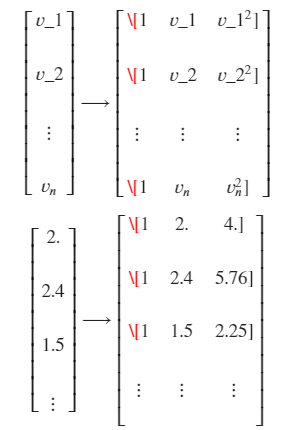
\includegraphics[scale=0.5]{figures/W1-matrix.png}
		\label{W301c-clone}
	\end{figure}
	
	It looks like feature sets for multiple linear regression analysis, right? Yes. It Does. Indeed, Polynomial regression is a special case of linear regression, with the main idea of how do you select your features.
	
	Just consider replacing the  $x$  with  $x_{1}$ , $x^{2}$  with  $x_{2}$ , and so on. Then the degree 2 equation would be turn into:
	
	\begin{equation}
		\hat{y} = b + \theta_{1}x_{1} + \theta_{2}x_{2}
	\end{equation}

	Now, we can deal with it as 'linear regression' problem. Therefore, this polynomial regression is considered to be a special case of traditional multiple linear regression. So, you can use the same mechanism as linear regression to solve such a problems.
	
	so we can use LinearRegression() function to solve it:
	
	\begin{verbatim}
		clf = linear_model.LinearRegression()
		train_y_ = clf.fit(train_x_poly, train_y)
		# The coefficients
		print ('Coefficients: ', clf.coef_)
		print ('Intercept: ',clf.intercept_)
		
		#Coefficients:  [[ 0.         50.14228586 -1.47509466]]
		#Intercept:  [107.48765006]
	\end{verbatim}

	As mentioned before, Coefficient and Intercept , are the parameters of the fit curvy line. Given that it is a typical multiple linear regression, with 3 parameters, and knowing that the parameters are the intercept and coefficients of hyperplane, sklearn has estimated them from our new set of feature sets. Lets plot it:
	
	\begin{verbatim}
		plt.scatter(train.ENGINESIZE, train.CO2EMISSIONS,  color='blue')
		XX = np.arange(0.0, 10.0, 0.1)
		yy = clf.intercept_[0]+ clf.coef_[0][1]*XX+ clf.coef_[0][2]*np.power(XX, 2)
		plt.plot(XX, yy, '-r' )
		plt.xlabel("Engine size")
		plt.ylabel("Emission")
		
		#Text(0, 0.5, 'Emission')
	\end{verbatim}

	\subsubsection{Evaluation}
	
	\begin{verbatim}
		from sklearn.metrics import r2_score
		
		test_x_poly = poly.fit_transform(test_x)
		test_y_ = clf.predict(test_x_poly)
		
		print("Mean absolute error: %.2f" % np.mean(np.absolute(test_y_ - test_y)))
		print("Residual sum of squares (MSE): %.2f" % np.mean((test_y_ - test_y) ** 2))
		print("R2-score: %.2f" % r2_score(test_y,test_y_ ) )
		
		#Mean absolute error: 24.74
		#Residual sum of squares (MSE): 991.48
		#R2-score: 0.77		
	\end{verbatim}
	
	
	\subsection{Lab: Non-linear Regression}